%% LaTeX-Beamer template for KIT design
%% by Erik Burger, Christian Hammer
%% title picture by Klaus Krogmann
%%
%% version 2.0
%%
%% mostly compatible to KIT corporate design v2.0
%% http://intranet.kit.edu/gestaltungsrichtlinien.php
%%
%% Problems, bugs and comments to
%% burger@kit.edu

\documentclass[18pt]{beamer}
\usetheme{kit}

%% TITLE PICTURE

% if a custom picture is to be used on the title page, copy it into the 'logos'
% directory, in the line below, replace 'mypicture' with the 
% filename (without extension) and uncomment the following line
% (picture proportions: 63 : 20, *.eps format if you use latex+dvips+ps2pdf,
% *.jpg/*.png/*.pdf if you use pdflatex)

%\titleimage{mypicture}

%% TITLE LOGO

% for a custom logo on the front page, copy your file into the 'logos'
% directory, insert the filename in the line below and uncomment it

%\titlelogo{mylogo}

% (*.eps format if you use latex+dvips+ps2pdf,
% *.jpg/*.png/*.pdf if you use pdflatex)

%% BIBTEX ICON/KEY

% if you want to see BibTeX keys in the references view instead of the symbol,
% uncomment the following line
% \usebibitemtemplate{\insertbiblabel}

% the presentation starts here

% change the following line to "ngerman" for German style date and logos
% change the following line to "english" for English style date and logos
\selectlanguage{ngerman}

\beamertemplatenavigationsymbolsempty

\usepackage{listings}
\definecolor{darkgray}{rgb}{0.95,0.95,0.95}
\definecolor{darkgreen}{rgb}{0.05,0.7,0.05}
\lstset{ language=Java,
	backgroundcolor=\color{darkgray}, 
	numbers=none, 
	keywordstyle=\color{black}\bfseries,
	tabsize=2,
	showspaces=false,               % show spaces adding particular underscores
	showstringspaces=false,         % underline spaces within strings
	showtabs=false, 
}



\title[Tutorium03]{Tutorium 03: Überschreiben und Überladen + Zustandsdiagramm}
\subtitle{Softwaretechnik im SS 2011, Tutorium 4}
\author{Jürgen Walter}
\date{\today}

\institute{Chair for Software Design and Quality}

\begin{document}

%title page
\begin{frame}
\titlepage
\end{frame}

%table of contents
\frame{
\frametitle{Was machen wir heute?}
	\tableofcontents
}

\section{Altes Übungsblatt}

\subsection{Altes Übungsblatt}
\frame {
\frametitle{Altes Übungsblatt}
	\begin{block}{Aufgabe 1: Sequenzdiagramm}
	\begin{itemize}
	\item Probleme mit Unterschied synchrone vs asynchrone Kommunikation
	\item Pfeilspitze ausmalen oder nicht?
	\end{itemize}
	\end{block}
}

\frame {
\frametitle{Altes Übungsblatt}
	\begin{block}{synchroner Nachrichten}
	\begin{itemize}
	\item Warten immer bis der aufgerufene fertig ist 
	\item (auch wenn keine Antworten gegeben werden)
	\end{itemize}
	\end{block}
	\pause

	\begin{block}{Antworten}
	\begin{itemize}
	\item nur bei synchronen Nachrichten möglich, optional
	\end{itemize}
	\end{block}
	\pause

	\begin{block}{asynchrone Nachrichten}
	\begin{itemize}
	\item "Mach es irgendwann zuende, ich bin nicht von dir abhängig!"
	\item z.B. Zerstörung eins Threads der nichts mehr tut, hier sollte das Programm nicht warten
	\item Entsprechen unsynchronisierten Thread-Operationen
	\item schneller, aber schwerer zu debuggen
	\end{itemize}
	\end{block}
}

\frame {
\frametitle{Altes Übungsblatt}
	\begin{block}{Sequenzdiagramm - Kommunikation}
	\begin{center}
	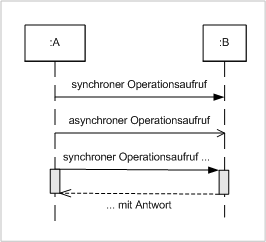
\includegraphics[width=0.6\textwidth]{pics/SequenzDiagramm1}
	\end{center}
	\end{block}
}

\frame {
\frametitle{Altes Übungsblatt}
	\begin{block}{Aufgabe 2: Zustandsdiagramm}
	\begin{itemize}
	\item Überwiegend richtig gelöst, sehr schön!
	\end{itemize}
	\end{block}
	\pause
	\begin{block}{Aufgabe 3:  Grafische Oberfläche für Floyd-Steinberg} 
	\begin{itemize}
	\item Bisher noch nicht korrigiert
	\end{itemize}
	\end{block}
}

\subsection{Zum Aufwärmen ...}
\frame {
\frametitle{Wahr oder falsch?}
\begin{itemize}
	\color<2->[rgb]{1,0,0}
	\item Implementierungsvererbung ist die Voraussetzung für Signaturvererbung 
	\color[rgb]{0,0,0}
	\pause
	\color<3->[rgb]{0,1,0}
	\item Ein Modul ist eine Menge von Programmelementen, die nach dem Geheimnisprinzip gemeinsam entworfen und geändert werden.
	\color[rgb]{0,0,0}
	
	\pause
	\color<4->[rgb]{1,0,0}
	\item Wenn eine Benutzthierarchie nur transitive Zyklen aufweist, heißt sie Benutztrelation
	\color[rgb]{0,0,0}
	\pause
	\color<5->[rgb]{1,0,0}
	\item Software ist leichter zu ändern als ein physisches Produkt vergleichbarer Komplexität.
	\color[rgb]{0,0,0}
	\pause
	\color<6->[rgb]{1,0,0}
	\item In Java muss eine abstrakte Klasse, die eine Schnittstelle implementiert, alle in der Schnittstelle vorgegebenen Methoden implementieren
	\color[rgb]{0,0,0}

\end{itemize}
}

\frame {
\frametitle {Klausuraufgaben zum Aufwärmen} 
	\begin{block} {Aufgabe 1 (2P)}
	Nennen Sie 4 aus der Vorlesung bekannte Techniken zur Anforderungsermittlung während der 			
	Planungsphase. \\
	\visible<2-> {
	\begin{itemize}
		\item Fragebögen (engl. questionnaires)
		\item Interviews
		\item Aufgaben-
		\item Dokumenten-
		\item Systemanalyse
		\item Szenarien (engl. scenarios)
		\item Anwendungsfälle (engl. use cases)
	\end{itemize}
	}
	\end{block}
}

\frame {
\frametitle {Klausuraufgaben zum Aufwärmen} 
	\begin{block} {Aufgabe 2 (1,5P)}
	Nennen Sie 3 Ergebnisartefakte der Planungsphase.\\
	\visible<2-> {
	\begin{itemize}
		\item Durchführbarkeitsstudie
		\item Lastenheft
		\item Projektkalkulation
		\item Projektplan
	\end{itemize}
	}
	\end{block}
}

\frame {
\frametitle {Klausuraufgaben zum Aufwärmen} 
	\begin{block} {Aufgabe 3 (1,5P)}
	Für welche vier Eigenschaften steht der Begriff „ACID“-Prinzip? (2P)\\
	\visible<2-> {
	\begin{itemize}
		\item Atomicity
		\item Consistency
		\item Durability
		\item Isolation
	\end{itemize}
	}
	\end{block} 
}

\section{Überladen und Überschreiben}
\subsection{Kovarianz und Kontravarianz}

\frame {
\frametitle{Varianz}
	\begin{block}{Kovarianz, Kontravarianz und Invarianz im Überblick}
	\begin{center}
	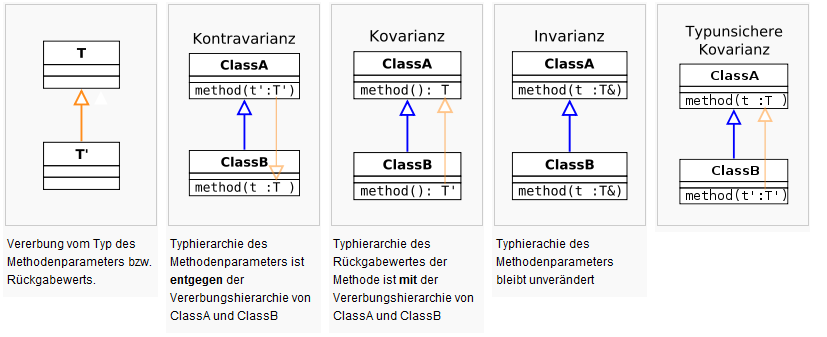
\includegraphics[width=1\textwidth]{pics/03/VarianzUeberblick}
	\end{center}
	\end{block}
}

\frame {
\frametitle {Varianz} 
	\begin{block} {Substitutionsprinzip / Liskovsches Substitutionsprinzip / Ersetzbarkeitsprinzip}
	" Objekte der abgeleiteten Klasse können stets Objekte der Oberklasse ersetzen"

	Durch das Substitutionsprinzip ergeben sich in der Polymorphie der objektorientierten Programmierung folgende 			Auftrittsmöglichkeiten für Varianzen:
	\visible<2-> {
	\begin{itemize}
		\item 	Kontravarianz  -  Eingabeparameter
		\item Kovarianz  - Rückgabewert und Ausnahmen
		\item Invarianz - Ein- und Ausgabeparameter

	\end{itemize}
	}
	\end{block} 
}


\begin{frame}[fragile]
\frametitle{Überladen}
	\begin{block}{Beispiel überladene Methoden}
	\begin{lstlisting}
		void printParameter(String p){
			System.out.println("Parameter = " + p);
		}
		void printParameter(char p){
			System.out.println("Parameter = " + p);
		}
		void printParameter(){
			System.out.println("no parameter passed");
		}
	\end{lstlisting}
	\end{block}
\end{frame}


\subsection{Überladen}
\frame {
\frametitle{Überladen}
	\begin{block}{Überladene Methoden}
	\begin{itemize}
	\item Methoden einer Klasse mit gleichen Namen, aber verschiedene Parameterlisten
	\item Bequem für den Benutzer
	\end{itemize}
	\end{block}
}


\subsection{Eclipse Demo}
\frame {
\frametitle{Eclipse Demo}
	\begin{block}{Themen}
	\begin{itemize}
	\item Vererbung
	\item Überladen
	\end{itemize}
	\end{block}
}


\section{UML}
\subsection{Zustandsdiagramm}

\frame{
\frametitle {Zustandsdiagramm (Wiederholung)} 
	\begin{itemize}
	\item Beschreibt mögliche Zustände eines Objekts sowie mögliche Zustandsübergänge
	\item Der Zustandsübergang (Transition) wird durch ein Ereignis ausgelöst
	\begin{center}
	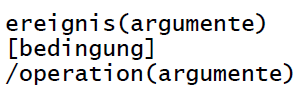
\includegraphics[scale=0.5]{pics/zustandsuebergang.png}
	\end{center}
	\item Zustandsübergang findet nur statt, wenn die Bedingung zu diesem Zeitpunkt erfüllt ist
	\item $\epsilon$ -Übergänge sind erlaubt
	\end{itemize}
}

\frame {
	\begin{exampleblock}{Zustandsdiagramm mit Gedächtnis (Wiederholung)}
	\begin{center}
	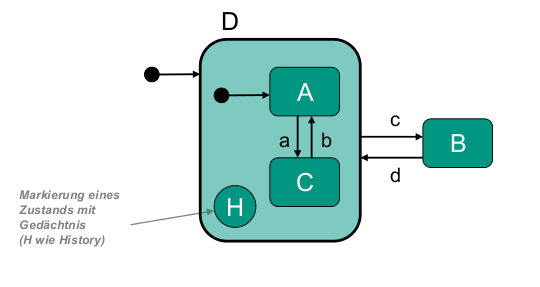
\includegraphics[scale=0.6]{pics/ZustandsDiagrammGedaechtnis.png}
	\end{center}
	\end{exampleblock}
}


\frame{
\frametitle {Klausuraufgabe 2009 (1P)}
	Gegeben ist der folgende UML-Zustandsautomat. Geben Sie an, in welcher Zustandskombination	
	sich der Zustandsautomat, jeweils ausgehend vom Startzustand, nach den beiden Eingabefolgen
	befindet. 
	\begin{itemize}
	\item Folge1: a, b, c, c   
	\visible<2-> {
	\item Zustandskombination: $A \times $D
	}
	\item Folge2: c, c, a, b, b, a, c, c, a
	\visible<3-> {
	\item Zustandskombination: $B \times $C
	}
	\end{itemize}
	\begin{center}
	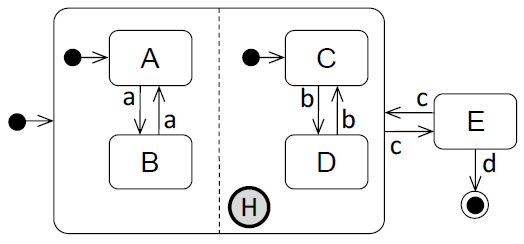
\includegraphics[scale=0.6]{pics/03/zustandN.png}
	\end{center}
}

\frame{
\frametitle {Klausuraufgabe 2009 (5P)}
	Wandeln Sie den UML-Zustandsautomaten in einen äquivalenten neuen um, der weder nebenläufige noch 				hierarchische Zustände oder Zustände mit Historie enthält. Leiten Sie die Namen für die Zustände wie folgt 			aus den Namen der Zustände des alten Automaten ab:
	\begin{itemize}
	\item Regel 1: Die Kombination der alten Zustände 1 und 2 wird zum neuen Zustand $1 \times 2$.
	\item Regel 2: Wurde der alte Zustand 1 vom alten Zustand 2 aus erreicht, ergibt dies den neuen
	Zustand 1(2). 
	\end{itemize}

	\begin{center}
	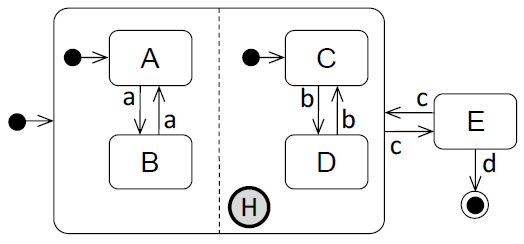
\includegraphics[scale=0.55]{pics/03/zustandN.png}
	\end{center}
}

\frame {
\frametitle {Musterlösung} 
	\begin{center}
	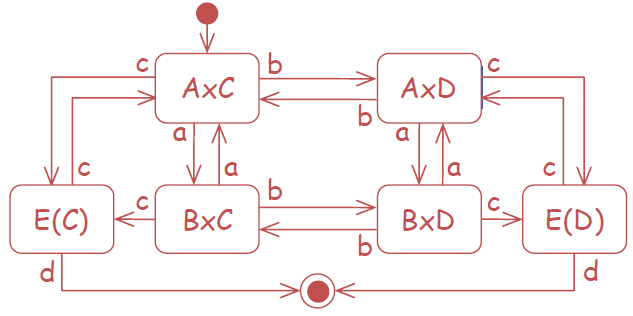
\includegraphics[scale=0.6]{pics/03/zustandNM.png}
	\end{center}
}

\section{Ende}
\subsection{Tipps zum nächsten Übungsblatt}

\frame{
\frametitle{Tipps zum nächsten Übungsblatt}

	\begin{block}{Aufgabe 1 - UML Zustandautomaten}
	\begin{itemize}
	\item a) Umkehrung der Klausuraufgabe des letzten Tutoriums
	\item b) Das History H gilt nur für den rechten Abschnitt
	\end{itemize}
	\end{block}

	\begin{block}{Aufgabe 2 - Überladen und Überschreiben}
	\begin{itemize} \pause
	\item Abgabe in der LEZ
	\item Vererbung ist das grundlegende Konzept der objektorientierten Programmierung
	\item Hier könnt ihr relativ schnell merken, ob ihr es verstanden habt!
	\end{itemize}
	\end{block}
}


\frame{
\frametitle{Tipps zum nächsten Übungsblatt}
	\begin{block}{Aufgabe 3 - Programmieren}
	\begin{itemize}
	\item Einfügen des der letzten Programmieraufgabe in JMRST
	\item TODO Wo muss ich was einfügen
	\item Wichtig: Sprache muss in eine Property Datei ausgelagert werden
	\end{itemize}
	\end{block}
}

\frame{
\frametitle{Tipps zum nächsten Übungsblatt}
	\begin{block}{Bonusaufgabe - Kammerjäger}
	\begin{itemize}
	\item Für die, die sich nicht ausgelastet fühlen
	\item Viel Aufwand für 3 Punkte
	\item Nutzt Eclipse tools zum profilen
	\end{itemize}
	\end{block}
}


\frame{
\frametitle{Bis zum nächsten Mal}
	\begin{center}
	
\includegraphics[height=200pt]{pics/02_zeitmaschine}
	\end{center}
}


\end{document}
